All cold cables originating from inside the cryostat connect to the outside warm electronics through PCB board \fdth{}s
installed in the signal flanges that are distributed along the cryostat roof.
The TPC data rate per \dword{apa}, with an overall \num{32}:\num{321} MUX and eighty $\sim$1~Gbps data channels per \dword{apa},
is sufficiently low that the \dword{lvds} signals can be driven over copper twin-axial transmission lines.
Additional transmission lines are available for the distribution of \dword{lvds} clock signals and I$^2$C control information,
which are transmitted at a lower bit rate.
Optical fiber is employed externally from the \dwords{wib} on the signal flange to the \dword{daq} and slow control systems described in Chapter~\ref{ch:fdsp-daq} and Chapter~\ref{ch:fdsp-slow-cryo}, respectively.

\begin{dunefigure}
[TPC \dword{ce} \fdth.]
{fig:tpcelec-signal_FT}
{TPC \dword{ce} \fdth. The \dwords{wib} are seen edge-on in the left panel, and in an oblique side-view in the right panel, which also shows the warm crate for a \dword{spmod} %DUNE module 
in a cutaway view.}
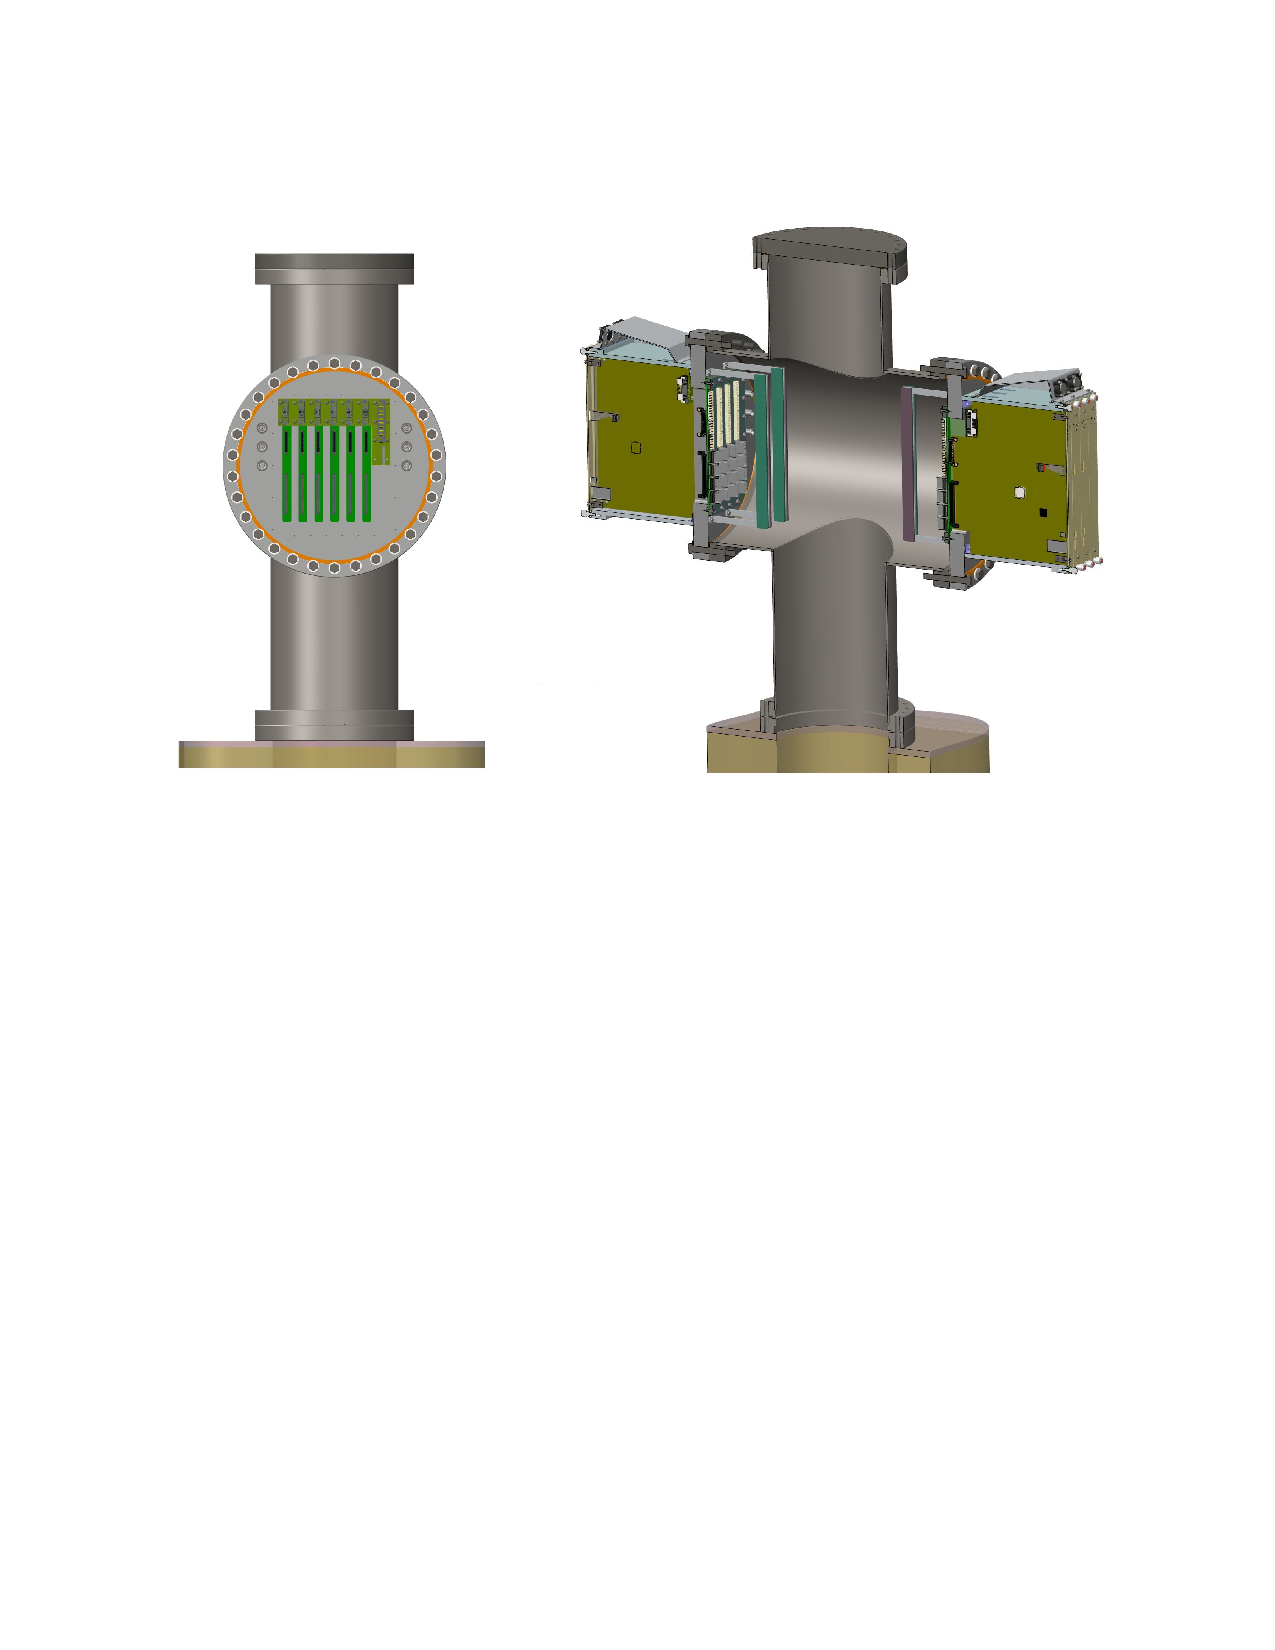
\includegraphics[width=0.9\linewidth]{tpcelec-signal_FT.pdf}
\end{dunefigure}

The design of the signal flange includes a four-way cross spool piece, separate PCB \fdth{}s for the \dword{ce} and \dword{pds} cables, and
an attached crate for the TPC warm electronics, as shown in Figure~\ref{fig:tpcelec-signal_FT}.
The wire bias voltage cables connect to standard SHV (safe high voltage) connectors machined directly into the \dword{ce} \fdth,
ensuring no electrical connection between the wire bias voltages and other signals passing through the signal flange.
Each \dword{ce} \fdth serves the bias, power, and digital I/O needs of one \dword{apa}.  

Data and control cable bundles are used to send system clock and control signals from the 
signal flange to the \dword{femb}, stream the $\sim$\SI{1}{Gbps} high-speed data from the \dword{femb} to the signal flange.  Each \dword{femb} 
connects to a signal flange via one data cable bundle, leading to 20 bundles between one \dword{apa} and one flange.  Each data bundle contains 12 low-skew twin-axial cables with a drain wire, 
to transmit the following differential signals:

\begin{itemize}
    \item four \SI{1.28}{Gbps} data (two from each \dword{coldata});
    \item two \SI{64}{MHz} clocks (one input to each \dword{coldata});
    \item two fast command lines (one input to each \dword{coldata});
    \item three I$^2$C-like control lines (clock, data-in, and data-out); and
    \item one multipurpose \dword{larasic} output (temperature, reference voltage, or analog test output).
\end{itemize}

The \dword{lv} power is passed from the signal flange to the \dword{femb} by bundles of
20AWG twisted-pair wires. Half of the wires are power feeds; the others
are attached to the grounds of the input amplifier circuits, as described in Section~\ref{sec:fdsp-tpc-elec-design-bias}.
For a single \dword{femb}, the resistance is measured to be  <\SI{30}{\milli\ohm} at room temperature or $<10$~m$\Omega$ at 
\lar temperature. Each \dword{apa} has a copper cross section of approximately %$80~\mathrm{mm}^2$ 
\SI{80}{mm$^2$}, with a 
resistance <\SI{1.5}{\milli\ohm} at room temperature or $<0.5$~m$\Omega$ at \lar temperature.

The bias voltages are applied to the $X$-, $U$-, and $G$-plane wire layers, three \dword{fc} terminations, 
and an electron diverter, as shown in Figure~\ref{fig:CR-board}. The voltages are supplied 
through eight SHV connectors mounted on the signal flange. RG-316 coaxial cables carry the voltages 
from the signal flange to a patch panel PCB which includes noise filtering mounted on the top 
end of the \dword{apa}. 

From there, wire bias voltages are carried by single wires to 
various points on the \dword{apa} frame, including the CR boards, a small PCB mounted on or near 
the patch panel that houses a noise filter and termination circuits for the field cage voltages, and 
a small mounted board near the electron diverter that also houses wire bias voltage filters.
